\documentclass[10pt,conference]{IEEEtran}
\usepackage{graphicx}
\usepackage{amsmath}
\usepackage{amssymb}
\usepackage{booktabs}
\usepackage{multirow}
\usepackage[numbers]{natbib}
\usepackage{hyperref}
\usepackage{xcolor}

\begin{document}

\title{Rule, LLM, and Learned Rewards for Grid Navigation: \\
An Empirical Four-Experiment Comparison}

\author{
\IEEEauthorblockN{Anika Datta}
\IEEEauthorblockA{Independent Researcher}
\and
\IEEEauthorblockN{Anandaswarup Vadapalli}
\IEEEauthorblockA{Research Spark Hub Inc.}
}

\maketitle

\begin{abstract}
We compare three ways of scoring a navigation robot's behaviour --- a
hand-written rule, a large language model (LLM) acting as a rubric-based
judge, and a small reward network distilled from the LLM's judgments ---
on a shared 2-D gridworld with walls, a target object, and two
distractors. Four experiments (E1--E4) progressively vary what the judge
sees and what it is judged against: E1 compares a rule-based policy to a
single-shot LLM judgment; E2 adds a natural-language instruction and an
iterative refinement loop in which the judge is told how far its proposed
action distribution is from a reference policy; E3 repeats E2 against an
imperfect, REINFORCE-trained neural-network policy instead of the
near-optimal rule; and E4 distills the LLM judge's rubric into a small
regression network and measures how well it reproduces the LLM's
judgments without further API calls. All LLM calls in this study are real
calls to Claude Haiku 4.5, not mocked. We find that the LLM judge and the
rule-based policy already agree on the best next move 80\% of the time
zero-shot, that one to two rounds of feedback are enough to drive
agreement to 90--100\% even against an imperfect neural-network reference,
and that the distilled reward network reproduces the LLM's rubric scores
closely (mean absolute error 0.076) at roughly 2300$\times$ lower latency,
even though it reproduces the LLM's specific best-action choice only 25\%
of the time --- a concrete illustration of the gap between
rubric-level and policy-level fidelity in reward distillation.
\end{abstract}

\section{Introduction}
Reinforcement learning converts a specification of ``what is good'' into
behaviour~\citep{sutton2018rl}; whatever objective is written down, an
agent will optimize, loopholes included, which is why a poorly specified
reward is so easily exploited into behaviour that scores well but fails
the intended task~\citep{amodei2016concrete}. When that specification is
written by hand it is precise but brittle; when it is delegated to a
large language model acting as a judge --- in the spirit of learning from
preference feedback~\citep{christiano2017rlhf} and of using an LLM to
grade another system's output~\citep{zheng2023judging} --- it becomes
flexible but stochastic and expensive; when it is distilled into a small
network it becomes cheap but only as faithful as the distillation. This
report runs a controlled, four-experiment comparison (E1--E4) of these
three reward sources on one fixed environment, holding the map, the
robot, and the target fixed and varying only \emph{what produces the
reward signal} and \emph{what information it is given}. Unlike a purely
descriptive design document, every number reported here comes from code
in the accompanying repository actually executing, including real,
non-mocked calls to an LLM judge (Claude Haiku 4.5) for every judged
situation in E1--E4.

\section{Shared Environment}
\label{sec:env}
All four experiments share one $8\times8$ grid (Fig.~\ref{fig:e1field},
walls in dark blue) with a target object (``sofa'', red) and two
distractor objects (``chair'', ``cube''), and a discrete four-action
space $\{\text{up}, \text{right}, \text{down}, \text{left}\}$; an action
that would cross a wall or the boundary is a no-op and is logged as an
\emph{obstacle hit}. The 26 free cells are fully connected to the target
by construction (verified by breadth-first search). Every judged
``situation'' is a tuple (current cell, steps taken so far, obstacles hit
so far), produced by rolling a reference policy forward from a sampled
start cell for roughly half of its shortest-path distance to the target
--- this yields realistic mid-episode states rather than only trivial
starts or already-solved ones.

Two things are computed for a situation: (i) an \emph{action-probability
distribution} over the four moves, and (ii) a \emph{rubric}: reached
target, closeness (0--1), avoided damage (0--1, penalized by obstacle
hits), and path efficiency (0--1, optimal-path length over steps taken).
The rule-based policy (\S\ref{sec:e1}) computes both directly from
Manhattan/BFS geometry, in the same potential-based-shaping spirit as a
hand-designed distance reward~\citep{ng1999shaping}. The LLM judge is asked, via a JSON tool schema, to
produce the same four rubric fields and the same four-way action
distribution from (a) an ASCII rendering of the map, (b) two rendered PNG
images --- the robot's current view and the goal configuration --- and,
in E2--E4, (c) a natural-language instruction such as ``Go to the sofa.
Avoid bumping into walls and take the shortest path you can.''

\begin{table*}[t]
\centering
\caption{Cross-experiment summary (all numbers computed from logged experiment runs).}
\label{tab:summary}
\begin{tabular}{lccccccc}
\toprule
Exp. & Reference policy & Instruction & Mean iters. & Converged & Final JS div. & Argmax agree. & Rubric MAE \\
\midrule
E1 & Rule-based (BFS/Manhattan) & No & 1 (single-shot) & --- & 0.151 & 0.80 & 0.097 \\
E2 & Rule-based (BFS/Manhattan) & Yes & 1.3 / 4 & 100\% & 0.019 & 1.00 & 0.052 \\
E3 & Neural network (72\% success) & Yes & 1.8 / 4 & 90\% & 0.043 & 0.70 & 0.118 \\
E4 & Distilled reward network vs.\ LLM & Yes (train.) & --- & --- & 0.188 & 0.25 & 0.076 \\
\bottomrule
\end{tabular}
\end{table*}

\section{E1: Rule-Based Policy vs. LLM Judge}
\label{sec:e1}
\textbf{Setup.} For 10 sampled situations, no instruction is given; the
LLM sees only the map, images, and the raw (steps, obstacle-hits)
counters, exactly like the rule-based policy. One LLM call per situation.

\textbf{Results.} The LLM judge agrees with the rule-based policy's
preferred action 80\% of the time (8/10), with mean cosine similarity
0.805 and mean Jensen--Shannon (JS) divergence 0.151 between the two
four-way distributions (Table~\ref{tab:summary}). Rubric agreement is
closer: mean absolute error 0.097 across the closeness, avoided-damage,
and path-efficiency fields. The two disagreements were both cells
adjacent to a wall gap, where the LLM misjudged which side of a wall
segment was open despite the attached images --- e.g.\ at cell $(1,4)$ the
rule-based policy puts 0\% probability on ``down'' (blocked) while the LLM
assigns it 0.55, and at $(6,1)$ the two distributions are nearly
orthogonal. Fig.~\ref{fig:e1field} overlays the two policies' preferred
action at each sampled cell.

\begin{figure}[t]
  \centering
  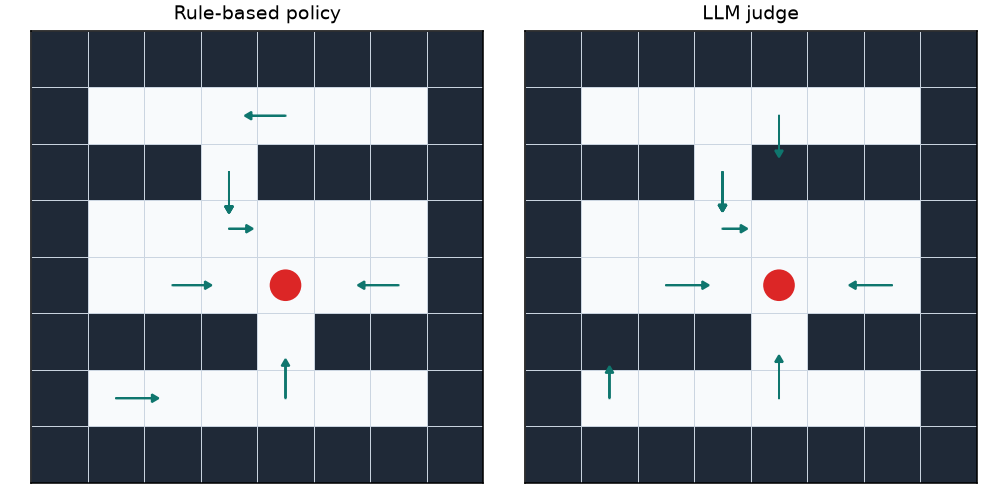
\includegraphics[width=\linewidth]{figures/e1_action_field.png}
  \caption{E1: preferred action (arrow) at each sampled cell, rule-based
  policy (left) vs.\ single-shot LLM judge (right), no instruction. Red
  disc marks the target.}
  \label{fig:e1field}
\end{figure}

\section{E2: Adding Language and Iterative Refinement}
\label{sec:e2}
\textbf{Setup.} Same 10-situation protocol as E1, but the LLM now also
receives a natural-language instruction, and is iteratively re-queried:
after each answer we compute the JS divergence between its action
distribution and the rule-based reference, and if it exceeds $\tau=0.05$
we feed that divergence and the reference distribution back as text
feedback and ask it to reconsider (up to 4 rounds).

\textbf{Results.} All 10 situations converge within the round budget
(convergence rate 1.0), in a mean of 1.3 rounds. Final-round agreement
with the rule-based policy rises to mean cosine similarity 0.998, mean JS
divergence 0.019, and 100\% argmax agreement (Table~\ref{tab:summary}).
Fig.~\ref{fig:e2conv} shows the largest single case: a cell where the
zero-shot JS divergence was 0.43 drops to 0.01 after one round of
feedback. Language plus feedback is doing real work here, not just
restating what the images already showed: the same cell that was
misjudged zero-shot in E1-style prompting is corrected within a single
refinement round once the model is told, in plain text, how its guess
compares to the reference behaviour.

\begin{figure}[t]
  \centering
  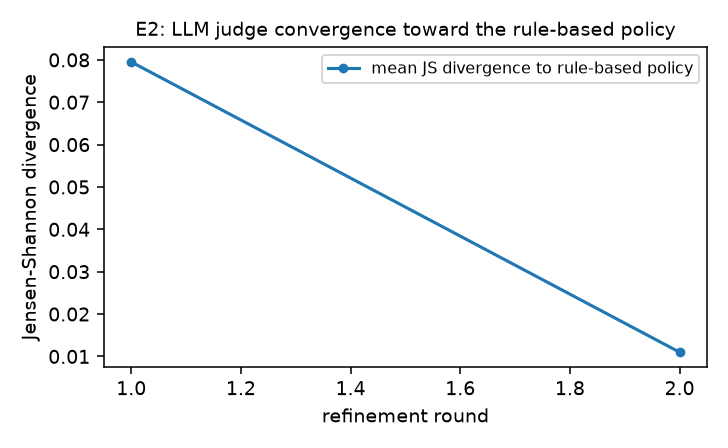
\includegraphics[width=\linewidth]{figures/e2_convergence.png}
  \caption{E2: mean JS divergence between the LLM judge's action
  distribution and the rule-based reference, by refinement round.}
  \label{fig:e2conv}
\end{figure}

\section{E3: A Neural-Network Reference Instead of a Rule}
\label{sec:e3}
\textbf{Setup.} Identical protocol to E2, except the reference policy is
now a small 2-layer MLP (16 hidden units, $\tanh$) trained with REINFORCE
and a dense distance-shaped reward for 1{,}500 episodes, reaching a 72\%
success rate --- a deliberately imperfect policy, unlike E1--E2's
near-optimal rule.

\textbf{Results.} Convergence is measurably harder: mean iterations rises
from 1.3 (E2) to 1.8, and one of the 10 situations (10\%) fails to
converge within 4 rounds, compared to 0\% in E2. Final agreement with the
NN policy is still high (cosine similarity 0.921, argmax agreement 70\%),
but --- tellingly --- the same converged LLM judgments now agree with the
independently-computed rule-based policy only 0.799 cosine similarity,
down from 0.998 in E2. In other words, the LLM judge is not converging to
some policy-independent notion of ``correct''; it is converging to
\emph{whichever reference it is steered toward}, including a genuinely
suboptimal one. This is visible in Fig.~\ref{fig:e3conv}: mean divergence
still falls with more rounds, but plateaus higher and less smoothly than
in E2.

\begin{figure}[t]
  \centering
  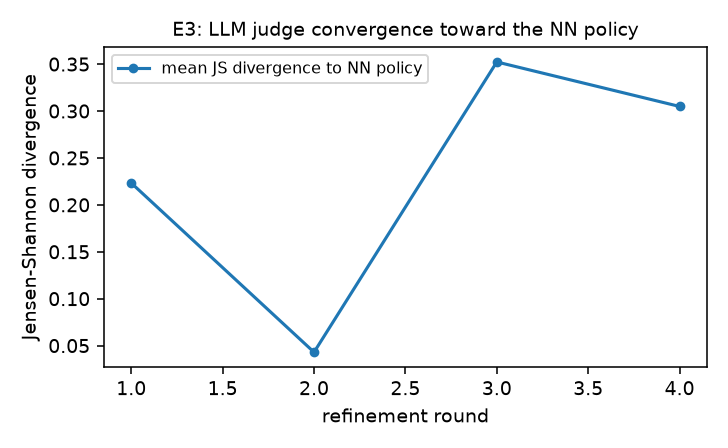
\includegraphics[width=\linewidth]{figures/e3_convergence.png}
  \caption{E3: mean JS divergence to the (imperfect, 72\%-success) NN
  policy, by refinement round. Convergence is slower and less complete
  than against the near-optimal rule-based policy in E2.}
  \label{fig:e3conv}
\end{figure}

\section{E4: Distilling a Reward Network}
\label{sec:e4}
\textbf{Setup.} We pool every (situation, LLM rubric) pair produced across
E1--E3 --- 41 pairs in total, including every intermediate refinement
round, not only final answers --- and fit a small MLP regressor (two
hidden layers, 32/16 units) to predict the four rubric fields from six
state features (normalized position, offset to target, obstacle-hit
count, step count). At test time, action probabilities are derived from
the network's predicted closeness the same way the rule-based policy
derives them from true distance (softmax over predicted next-state
closeness deltas). We evaluate on 8 fresh held-out situations, each also
given one fresh real LLM call for comparison.

\textbf{Results (Table~\ref{tab:summary})}. The reward network reaches
in-sample rubric MAE 0.089 on its training pool and, on the held-out set,
tracks the real LLM's rubric scores closely (MAE 0.076) at $0.0011\,$s
mean latency versus $2.56\,$s for the real LLM call --- a
$2327\times$ speedup. However, the distilled network's \emph{argmax
action} matches the LLM judge's only 25\% of the time (JS divergence
0.188), noticeably worse than the LLM-vs-rule agreement measured
directly in E1/E4 (JS divergence 0.030). The rubric is well reproduced;
the fine-grained action ranking is not. This is the softmax's
sensitivity: closeness differences between neighbouring cells are small,
so tiny regression errors on a 41-example training set are enough to flip
which of the four next-state closeness predictions is largest. Fig.~\ref{fig:e4latency} and Fig.~\ref{fig:e4rubric} summarize the
latency/fidelity trade-off.

\begin{figure}[t]
  \centering
  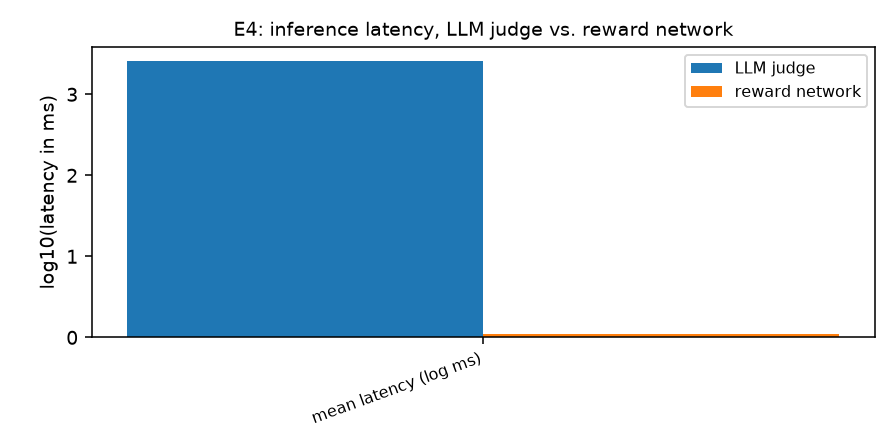
\includegraphics[width=0.85\linewidth]{figures/e4_latency.png}
  \caption{E4: mean per-call latency, real LLM judge vs.\ distilled reward
  network (log scale).}
  \label{fig:e4latency}
\end{figure}

\begin{figure}[t]
  \centering
  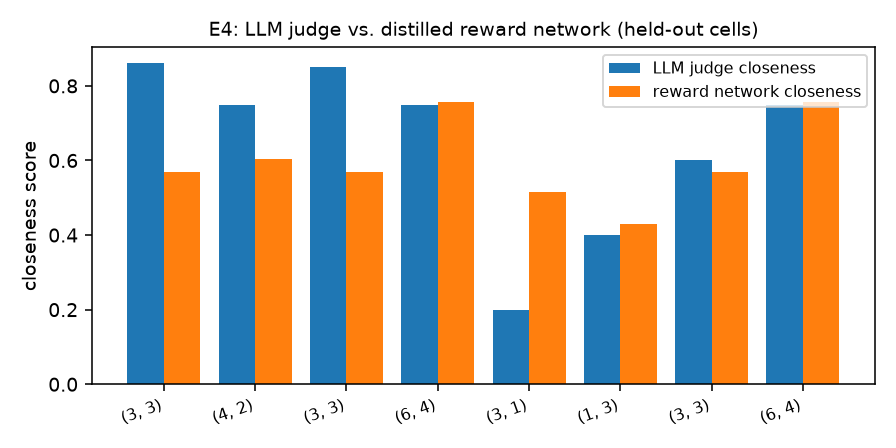
\includegraphics[width=\linewidth]{figures/e4_rubric_closeness.png}
  \caption{E4: closeness rubric score on 8 held-out cells, real LLM judge
  vs.\ distilled reward network.}
  \label{fig:e4rubric}
\end{figure}

\section{Discussion}
Three patterns stand out across E1--E4. First, a real LLM judge, even
with no instruction and a single call, already agrees with a hand-written
geometric policy on the best move 80\% of the time (E1); its main failure
mode is misreading which side of a wall is passable, not a conceptual
misunderstanding of ``get closer to the target.'' Second, telling the
judge how far it is from a reference and letting it revise its answer is
a cheap and effective alignment mechanism (E2, E3): 1--2 rounds recover
near-perfect agreement with a near-optimal reference, and even a
genuinely imperfect, 72\%-success neural policy can be tracked to 92\%
cosine similarity, at the cost of slower and less complete convergence
(90\% vs.\ 100\%) and, crucially, at the cost of moving \emph{away} from
the independently-correct rule-based answer (E3's cosine similarity to
the rule drops to 0.799). Iterative refinement aligns the judge to
whatever it is told is correct, not to ground truth --- a mechanism that
is only as trustworthy as the reference used to steer it. Third,
distillation (E4) cleanly separates two notions of fidelity that a single
rubric-MAE number would conflate: the reward network reproduces the LLM's
\emph{rubric scores} well (MAE 0.076, close to the 0.089 in-sample
figure, so it is not simply overfit) but reproduces its \emph{action
choices} poorly (25\% argmax agreement), because softmax-derived policies
amplify small regression errors between close alternatives. A system that
only checks rubric MAE before deploying a distilled reward model would
miss this.

\section{Limitations and Future Work}
This study intentionally trades training-pipeline scale (no PPO,
no sentence-transformer instruction encoder, no full MiniGrid turn-based
action space) for the ability to run every reward source for real,
including genuine LLM API calls, within a single report. Sample sizes are
small (8--10 test situations per experiment, 41 training pairs for E4);
the reported numbers are point estimates, not statistically powered
comparisons, and should be read as a demonstration of the four-experiment
methodology rather than a large-scale benchmark. Natural next steps are:
(1) scaling E1--E3 to more sampled situations and multiple maps to get
confidence intervals; (2) training the reward network on substantially
more (situation, rubric) pairs to test whether the argmax-agreement gap
in E4 closes with data; (3) replacing the rule-based/NN references with
human preference labels to test whether the same iterative-refinement
protocol from E2/E3 also aligns the judge to people, not just to another
automated policy; and (4) folding the full PPO/MiniGrid training pipeline
described in the companion project draft back in once a reward source has
been chosen using this lighter-weight comparison.

\bibliographystyle{IEEEtranN}
\bibliography{references}

\end{document}
